\section{Zielsetzung}
Das Ziel des vorliegenden Versuches ist es, sich anhand von Monte-Carlo-Simulationsdaten mit Methoden der Neutrinoselektion am IceCube-Experiment vertraut zu machen. Zum Durchführen der Seperation werden verschiedene Methoden des Maschinellen Lernens verwendet.
\section{Theorie}
\label{kap:Theorie}
Die aktuellen Erkenntnisse in der Astrophysik basieren darauf, dass im 20. Jahrhundert die optische Astronomie auf andere Wellenlängenbereiche erweitert werden konnte. Heutzutage werden neben dem optischen Bereich, auch Radio-, Röntgen-, Infrarot-, und Ultraviolettastronomie entwickelt.\\
Entscheidend ist zudem die durch Victor Heß im Jahre 1912 entdeckte Höhenstrahlung. Sie war bis in die 1950er Jahre die einzige Quelle hochenergetischer Teilchen. Ihre Entdeckung zeigte, dass die Erde bzw. die Atmosphäre neben Photonen auch von anderen Teilchen getroffen wird. Beim Auftreffen der geladenen kosmischen Strahlung, der sogenannten Primärteilchen, kommt es zur Wechselwirkung mit der Atmosphäre, sodass Teilchenkaskaden aus Sekundärteilchen entstehen. Diese lassen sich über verschiedene Methoden abhängig von ihren Teilcheneigenschaften nachweisen. Die geladene kosmische Strahlung setzt sich neben Protonen aus Helium und anderen schweren Kernen zusammen, wobei die genau Zusammensetzung von dem Energiebereich abhängt. Dieses Spektrum wird durch ein Potenzgesetz beschrieben:
\begin{align}
	\frac{\text{d}\Phi}{\text{d}E} = \Phi_{0} \cdot E^{\gamma}
\end{align}
Der spektrale Index $\gamma$ liegt für die geladene Höhenstrahlung bei $\gamma \approx -2.7$. Dies liegt vor allem daran, dass geladene Materie auf ihrem Weg zur Erde durch galaktische und extragalaktische Magnetfelder abgelenkt werden. Dies verhindert eine Richtungsrekonstruktion, sodass auch ihre Quellen bisher unbekannt sind.
\subsection{Klassifizierung von Leptonen}
Bei IceCube werden Leptonen, hauptsächlich Myonen und Neutrinos, untersucht. Diese können sowohl aus der Höhenstrahlung, als auch astrophysikalischen Quellen stammen und unterscheiden sich durch ihre Energieverteilung und damit dem spektralen Index. \\
Die Atmosphärischen Myonen und Neutrinos werden außerdem in Konventionelle und Prompte unterschieden. Die Konventionellen entstehen, wenn bei der Wechselwirkung der geladenen kosmischen Strahlung Pionen oder Kaonen erzeugt werden. Durch ihre teilweise lange Lebensdauer verlieren diese Mesonen Energie, bevor sie in die konventionellen Myonen bzw. Neutrinos zerfallen. Daher gilt für das Spektrum der konventionellen Myonen und Neutrinos $\propto E^{-3.7}$.\\
Bei der Wechselwirkung der geladenen kosmischen Strahlung mit der Atmosphäre können jedoch auch kurzlebige, schwere Hadronen, wie $D$-Mesonen oder $\Lambda_{c}$-Baryonen entstehen. Diese zerfallen ohne nennenswerte Energieverluste weiter in die promten Myonen und Neutrinos. Daher ist deren Spektrum  $\propto E^{-2.7}$ und somit direkt vererbt von der geladenen kosmischen Strahlung.\\
Es wird davon ausgegangen, dass astrophysikalische Quellen, die Hadronen beschleunigen, auch Neutrinos und hochenergetische Photonen emittieren. Da sie ungeladen sind, werden sie nicht durch äußere Magnetfelder abgelenkt und liefern somit Informationen über ihren Ursprung. Der Vorteil von Neutrinos im Gegensatz zu Photonen ist, dass sie durch ihren sehr kleinen Wirkungsquerschnitt ebenfalls Staubwolken und optisch dichte Medien durchdringen können und somit Informationen über das optisch dichtere Innere eines astrophysikalischen Objektes liefern. Unter Annahme von Stoßbeschleunigung nach Fermi \cite{PhysRev.75.1169}, besitzt der astrophysikalische Neutrinofluss einen spektralen Index von  $\propto E^{-2}$.\\
\subsection{Das IceCube-Experiment}
Das IceCube-Experiment wird zur Detektion von hochenergetischen Neutrinos und Myonen genutzt. Es befindet sich am geographischen Südpol in einer Tiefe von $1450-\SI{2450}{\meter}$ unter der Oberfläche in einer klaren Eisschicht. Insgesamt setzt sich der Detektor aus den drei Komponenten Ice-Top \cite{3246225}, In-Ice-Array \cite{ACHTERBERG2006155} und DeepCore \cite{2143409} zusammen. Eine schematische Darstellung des Detektors befindet sich in Abbildung \ref{fig:Ice}.
\begin{figure}
  \centering
  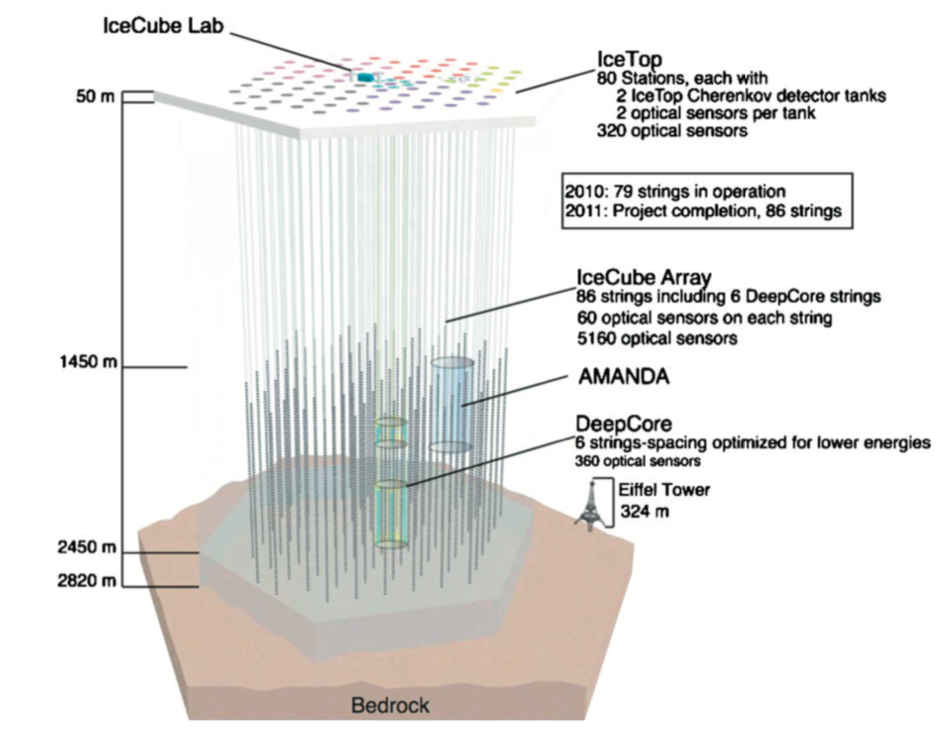
\includegraphics[width=0.5\textwidth]{graphics/IceCube.png}
  \caption{Schematische Darstellung des IceCube-Detektors mit seinen drei Komponenten Ice-Top, In-Ice-Array und DeepCore.\cite{IceCube}}
  \label{fig:Ice}
\end{figure}
Zu Teilchendetektion wird sich dabei das Prinzip von Tscherenkov-Licht zu nutze gemacht. Dieses wird emittiert, wenn sich ein hochenergetisches, geladenes Teilchen überlichtschnell im Medium bewegt. Die Lichtgeschwindigkeit im Medium ist $c=\frac{c_{0}}{n}$, wobei $n$ dem Brechungsindex des Mediums entspricht und $c_{0}$ der Vakuumlichtgeschwindigkeit. Dieses Tscherenkov-Licht kann mit 5160 Photoelektronenvervielfachern aufgenommen werden, die auf insgesamt 86 Kabel verteilt sind.\\
Diese bilden grundsätzlich das In-Ice-Array, das eine Energieschwelle von $\SI{100}{\giga\electronvolt}$ besitzt. Der DeepCore besteht aus 7 mittig liegend Kabeln der insgesamt 86 Kabel, die dichter zusammenliegen und eine höhere Photomultiplierdichte besitzen. Daher bildet er die Niederenergieerweiterung des Detektors und hat eine Energieschwelle von bereits $\SI{10}{\giga\electronvolt}$.\\
Das IceTop ist ein Luftschauer-Experiment aus lichtdichten Eistanks. Es dient mithilfe von Tscherenkov-Licht sowohl zur Untersuchung von kosmischer Strahlung als auch als Veto für das In-Ice-Array. So können zum Beispiel atmosphärische Teilchen von Neutrinos, die die Erde durchquert haben, unterschieden werden.\\
Neutrinos lassen sich bei IceCube über die Sekundärteilchen aus schwacher Wechselwirkung detektieren. Dabei existieren geladene Ströme (\textit{engl.: charged currents}, CC) und neutrale Ströme (\textit{engl.: neutral currents}, NC), die wie folgt aussehen:\\
\begin{align}
	\nu_{l}(\bar{\nu_{l}}) + A \to l^{\mp} + X (\text{CC})\\
	\nu_{l} + A \to \nu_{l} + X (\text{NC})
\end{align}
Elektronen produzieren auf Grund ihrer geringen Energie einen nahezu sphärischen Schauer im Detektor. Ähnlich verhält es sich für Tau-Leptonen, die auf Grund ihrer kurzen Lebensdauer auch nur eine geringe Reichweite haben, bevor sie zerfallen. Bei nicht zu hohen Energien ähnelt die Signatur somit stark der von Elektronen. \\
Myonen hingegen haben eine lange Spur, dies liegt an ihrem deutlich langsameren Energieverlust und der daraus resultierenden großen Reichweite. Das Tscherenkov-Licht der Myonen selbst ist jedoch zu schwach zur Detektion. Sie werden durch die Schauer der emittierten Photonen und Elektron-Positron-Paare detektiert.\\
Bei den schwachen Wechselwirkungen über neutrale Ströme werden die Kaskaden ausgelöst durch die hadronischen Sekundärteilchen beobachtet. Diese ähneln stark der durch Elektronen ausgelösten Schauer.

\subsection{Messungen von Neutrinos mit IceCube}
Bei der Messung von Ereignissen wird grundsätzlich zwischen zwei verschiedenen Arten unterschieden. Zum einen den sogenannten \textit{starting events}, die erst im Detektor selber entstehen und zum anderen, den Myon-Ereignissen, die den gesamten Detektor durchqueren. Der Vorteil dabei ist, dass diese zwar im Vergleich zu den \textit{starting events} eine schlechtere Energieauflösung besitzen, aber eine deutlich bessere Winkelauflösung. Die Selektion bei den beiden Ereignisarten unterscheidet sich jedoch grundlegend.\\
Die Analysetechnik bei den \textit{starting events} nutzt den äußeren Abschnitt des Detektors als Veto, um atmosphärische Myonen zu verwerfen. Da alle Neutrinoflavour gleicher Maßen beitragen, stammen ein Großteil der Ereignisse aus Kaskaden von Wechselwickungen über den neutralen Strom oder Elektron- und Tauwechselwirkungen über den geladenen Strom.\\
Bei den durchquerenden Myon-Ereignissen kann das effektive Volumen für die Analyse erweitert werden, indem die Erde als Abschirmung von atmosphärischen Myonen genutzt wird. Myonen, die von unterhalb des Detektors kommen, stammen somit aus Neutrinowechselwirkungen. Somit ermöglicht ein Schnitt im Zenitwinkel das Trennen von atmosphärischen Myonen und Myonen aus Neutrinowechselwirkungen. Ein Teil der Richtungsrekonstruktion verläuft jedoch fehlerhaft, sodass der Schnitt auf den rekonstruierten Zenitwinkel nur eine Verbesserung vom Signal-Untergrund-Verhältnis von $1:10^{6}$ auf $1:10^{3}$ bringt. Um das Signal-Untergrund-Verhältnis weiter zu verbessern, werden Methoden des Maschinellen Lernens verwendet.

\subsection{Signal-Untergrund-Trennung mit Maschinellen Lernen}
\label{Signal}
Um Methoden des Maschinellen Lernens für die Signal-Untergrund-Trennung nutzen zu können, müssen diese zunächst auf Monte-Carlo-Testdatensätze angewendet werden. Dazu werden zunächst Signal und Untergrund getrennt von einander simuliert. Um ein möglichst einheitliches Bild für beide Datensätze zu erhalten, werden alle Attribute, die nur in einem der beiden Datensätze vorkommen, entfernt. Zudem werden alle Monte-Carlo-Wahrheiten, Eventidentifikationsnummern und Gewichte entfernt. Um fehlerhafte Ergebnisse zu verhindern, müssen zudem Werte, die nicht als Zahl identifiziert werden können, wie zum Beispiel NaN oder Inf entfernt werden. Trifft das auf unter \SI{30}{\percent} der Werte eines Attributes zu, bietet es sich an, diese durch eine alternative Zahl, die nicht im Wertebereich des Attributes liegt, zu ersetzen. Andernfalls sollte auch dieses Attribut verworfen werden. Zudem müssen Signal und Untergrund mit einem binären Label von einander unterschieden werden.\\
Da solche Datensätze oft eine Vielzahl an Attributen besitzen, bei denen zudem der Informationsgehalt in Bezug auf die Zielklasse sehr stark schwankt, bietet es sich an, zuvor eine Attributsselektion durchzuführen. Damit wird die Laufzeit der multivarianten Lerner stark verringert. Ein mögliches Verfahren zur Attributsselektion ist die \textit{Forward Selection}.
\subsubsection{Vorwärtsauswahl}
Die Vorwärtsauswahl (\textit{engl.: Forward Selection}) arbeitet iterativ und ist abhängig von dem verwendeten Lerner. Dieser erzeugt ein Modell, welchem die Vorwärtsauswahl iterativ die Variable hinzufügt, welche zusammen mit den bereits ausgwählten Variablen die Vorhersagekraft des Modells am meisten erhöht.
\subsubsection{Stabilitätsanalyse mit dem Jaccard-Index}
Statistische Schwankungen im Lerner können die Stabilität der Attributsauswahl beeinträchtigen. Diese Stabilität lässt sich mit dem Jaccard-Index untersuchen, welcher ein Maß für die Ähnlichkeit zweier Teilmengen $F_{a},F_{b}$ ist. Er wird definiert über:
\begin{align}
	J(F_{a},F_{b}) = \frac{|F_{a} \cup F_{b}|}{|F_{a} \cap F_{b}|}
\end{align}
Der Index $\hat{J}$ erlaubt die Ähnlichkeit verschiedener Selektionen zu beurteilen. Dazu wird der Datensatz in $l$ Teilmengen auf geteilt, auf denen $l$-mal die Attributsauswahl durchgeführt wird. Dadurch ergibt sich der Index $\hat{J}$ zu:
\begin{align}
	\hat{J} = \frac{2}{l(l-1)} \sum^{l}_{i=1} \sum^{l}_{j=i+1} J(F_{i},F_{j})
	\label{eq:jc}
\end{align}

Die Attributsauswahl ist stabil gegenüber statistischen Schwankungen, wenn der Wert nahezu $1$ ergibt.
\label{jaccard}
% \subsubsection{mRMR-Auswahl}
% Die mRMR-Auswahl (\textit{engl.: minimum Redundancy, Maximum Relevance}) basiert auf der Betrachtung der Wahrscheinlichkeitsverteilungen der zur Verfügung stehend Varaiblen. Die mRMR-Selektion wählt dabei die Attribute iterativ aus, indem sie nach welchen sucht, die möglichst stark mit der Zielvariable, aber möglichst gering untereinander korreliert sind. Dabei nutzt sie unter anderem den gemeinsamen Informationsgehalt $I(x,y)$ zweier Variablen $x,y$:
% \begin{align}
% 	I(x,y) = \int p(x,y) \log\left(\frac{p(x,y)}{p(x)p(y)}\right)\text{d}x\text{d}y.
% \end{align}
% Wobei $p(x), p(y)$ und $p(x,y)$ die Wahrscheinlichkeitsverteilungen der betreffenden Variablen sind. Die Zielvariable des vorliegenden Versuchs ist dabei die Klasse des Ereignisses, also ob es sich um ein Signal- oder Untergrundereignis handelt.
\subsubsection{Verschiedene Lernalgorithmen}
Ein Lernalgorithmus ist der Naive-Bayes-Lerner, der auf dem Bayes'schen Theorem über bedingte Wahrscheinlichkeiten
\begin{align}
	p(A|B) = \frac{p(B|A)p(A)}{p(B)}
\end{align}
basiert. Wenn $A$ die Klassenzugehörigkeit ($A$ Signal, $\bar{A}$ Untergrund) bezeichnet und $B$ ein Attribut ist, dann gilt für den Audruck
\begin{align}
	Q = \frac{p(A|B)}{p(\bar{A}|B)} = \frac{p(B|A)p(A)}{p(B|\bar{A})p(\bar{A})},
\end{align}
dass er einen Wert von mehr als 1 annimmt, wenn das Ereignis mit größerer Wahrscheinlichkeit Signal und nicht Untergrund ist. Unter der naiven Annahme, dass Attribute nur von der Klassenzugehörigkeit abhängen, ergibt sich $Q$ mit mehreren Attributen zu:\\
\begin{align}
	Q = \frac{p(A|B_{1},...,B_{n})}{p(\bar{A}|B_{1},...,B_{n})} = \prod_{i=1}^{n} \frac{p(B_{i}|A)}{p(B_{i}|\bar{A})}
\end{align}
Der kNN-Klassifikator (\textbf{k} \textbf{N}ächste \textbf{N}achbarn) klassifiziert die Klasse eines Ereignisses, indem er die $k$ umliegenden Ereignisse betrachtet und das Ereignis anhand des Mittelwerts der umliegenden Ereignisse klassifiziert.\\
Ein dritter Klassifikator ist der Random Forest, der auf binären Entscheidungsbäumen basiert. Dabei wird an jedem Knoten eines Entscheidungsbaum ein Schnitt angewendet und die entstehenden Teilmengen werden auf die beiden Äste aufgeteilt. Dieses Verfahren wird entweder bis zu einer gewissen Tiefe fortgeführt oder bis die Blätter nur Ereignisse der selben Klasse enthalten.
Um die Effekte des Übertrainierens zu minimieren, kann über eine Menge unterschiedlicher Entscheidungsbäume gemittelt werden. Eine mögliche Strategie dafür ist, dass jeder Baum nur auf einer Teilmenge des Trainingsdatensatz trainiert wird und die $k$ Attribute für den Schnitt an jedem Knoten zufällig gewählt werden. Die Confidence $c$, also Entscheidung des Random Forst ist das arithmetische Mittel über die Entscheidungen $P_{i}$ der $N$ Einzelbäume.
\begin{align}
	c = \frac{1}{N} \sum_{i=1}^{N}P_{i} \; \text{mit} P_{i} \in \{0,1\}
\end{align}
\subsubsection{Qualitätsparameter}
Die Güte einer Klassifikation lässt sich mit den Qualitätsparametern bewerten. Diese basierten auf der Anzahl der korrekt als Signal (\textit{tp, true positiv}) bzw. Untergrund (\textit{tn, true negativ}) und der fälschlicher Weise als Signal (\textit{fp, false positiv}) bzw. Untergrund (\textit{fn, false negativ}) klassifizierten Ereignisse. Es lassen sich die beiden Parameter
\begin{align}
	\text{Reinheit}\, p &= \frac{tp}{tp+fp}\\
	\text{Effizienz}\, r &= \frac{tp}{tp+fn}
\end{align}
bestimmen. Wichtig ist dabei, dass je nach Ziel der Analyse einer der beiden Parameter optimiert wird. Ist zum Beispiel eine sehr reine Trennung sehr wichtig, aber es ist nicht wichtig für statistische Untersuchungen eine gewisse Anzahl an Ereignissen zu haben, bietet es sich an die Reinheit zu maximieren.
\subsubsection{Kreuzvalidierung}
Die Kreuzvalidierung ist ein Werkzeug, dass es ermöglicht einen Fehler auf die Qualitätsparameter anzugeben. Dieser entsteht auf Grund von statistischen Schwankungen im Trainingsdatensatz. Dazu wird der Trainingsdatensatz in $n$ Datensätze aufgeteilt. Von diesen Teildatensätzen werden $n-1$ zum trainieren des Lerners verwendet. Mit dem $n$-ten Datensatz wird schließlich die Klassifikation mit dem erhaltenden Lerner aufgestellt. Dieses Verfahren wird $n$-mal durchgeführt, sodass jeder Datensatz einmal Testdatensatz war. Aus den $n$ Qualitätsparametern lässt sich schließlich ein Mittelwert und der zugehörige Fehler auf diesen berechnen.
\subsubsection{Monte-Carlo-Simulationen}
Kann ein Experiment gar nicht oder nur sehr aufwendig analytisch beschrieben werden, bietet die Verwendung von Monte-Carlo-Simulationen eine Alternative. Dabei wird ein Experiment unter Verwendung von Zufallszahlen simuliert. \\
In der Teilchenphysik werden sie häufig zum Bereitstellen von Pseudodaten genutzt. Da die Eigenschaften der Signal- und Untergrundereignisse bekannt sind, bieten sie sich zum Beispiel zur Klassifizierung von Rekonstruktionsalgorithmen an. Analog können mit ihnen auch Analysen zur Signal-Untergrund-Trennung durchgeführt werden. Dieses Vorgehen wird in diesem Versuch durchgeführt.
